\documentclass{report_class}

\title{Basic Concepts of Solid-State Physics\\presented by the example of Calcium}
\subtitle{adf}
\author{Patrick Jenny 100639\\Filip Banasiak 100661}
\date{\today}

\begin{document}
	\maketitle
	\centerline{Group: G9}
	\pagenumbering{Roman}
	
	\tableofcontents
	\newpage
	
	\section*{ABSTRACT}
The goal of this report is to show the basic concepts of Solid-State Physics in general and especially for Calcium. In Chapter \ref{chap1} we will talk about Crystal Structure and how it is described, the lattice in which Calcium crystalyzed could be identified and basic properties derived
Chapter \ref{chap2} will provide further informations about how to determine these structures. Diffraction patters for Calcium could be derived.
To get further insides in the topic of Solid-State Physics in Chapter \ref{chap3}, we will discuss some of the models which are used to describe Atoms which are not at rest at their lattice site.


	\newpage

	\clearpage
	\pagenumbering{arabic}
	
	\section{Introduction}
	he goal of this report is to show the basic concepts of Solid-State Physics 
in general and especially for Calcium.
Calcium metal is used as a reducing agent in preparing other metals such as 
thorium and uranium. 
It is also used as an alloying agent for aluminium, beryllium, copper, lead 
and magnesium alloys.
These use cases make a deeper understanding of solids states essential.

In the FIRST CHAPTER we will talk about the Chrystal Structures and how they 
are described.
Most of the basic concepts will be shown directly by the example of calcium. 
The book \textit{Elementary Solid State Physics}
provided the necessary background information. In the SECOND CHAPTER we will 
talk about diffraction in this crystal,
as by studying the diffraction pattern of a beam information about the 
structure of the crystal can be obtained.
\textit{Elementary Solid State Physics} \cite{elementary_SSP} delivered insights in these concepts to get 
further information or different 
explanation to some topics, \textit{Introduction to Solid State Physics} \cite{kittel} was used in addition. 
In the first to parts, it is assumed that the Atoms stay at rest at their
position. In reality this is not true as atoms oscillate arround their
rest position. In CHAPTER 3 we will show some of these effecs.
	\newpage

	\section{Results}
		%------1-CHAPTER------%
		\section{Chapter 1}

\begin{figure}[H]
	\centering
	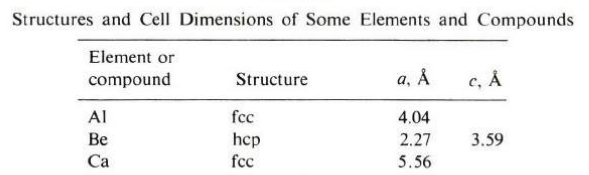
\includegraphics[width=0.7\linewidth]{Graphics/Chapter1/StructuresAndCellDimension_Table1_2_Omar}
	\caption{}
	\label{}
\end{figure}


\textbf{Unit Cell}
\begin{figure}[H]
	\centering
	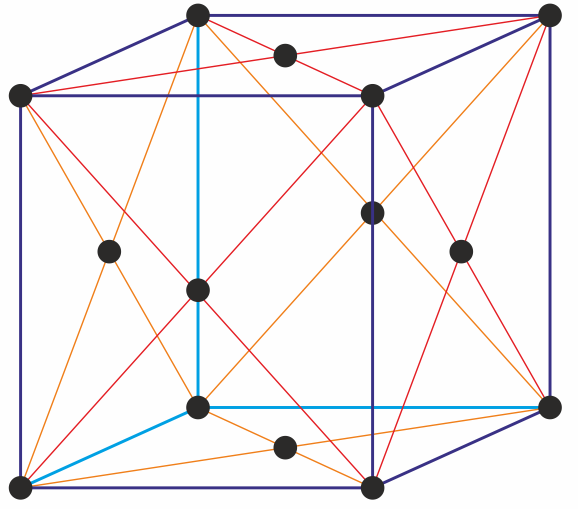
\includegraphics[width=0.4\linewidth]{Graphics/Chapter1/face-centered_cubic_lattice.png}
	\caption{FCC-Lattice}
	\label{}
\end{figure}

\textbf{Primitive Vectors}

The three primitive vectors are

\begin{figure}[H]
	\centering
	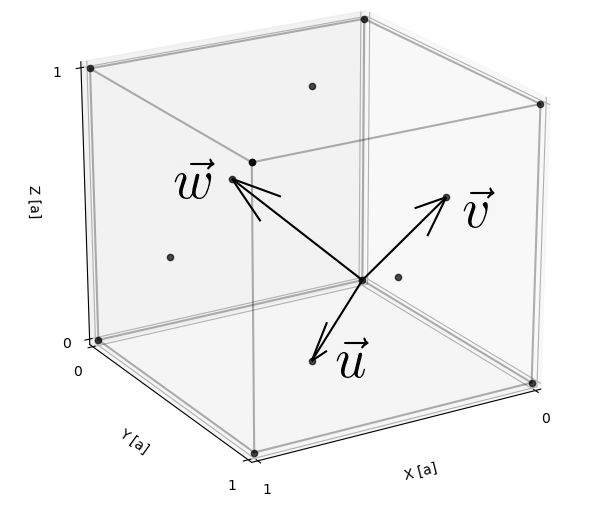
\includegraphics[width=0.5\linewidth]{Graphics/Chapter1/prim_vec}
	\caption{Primitive Vectors in a FCC-Lattice}
	\label{}
\end{figure}

$$\vec{u} = \frac{a}{2} \left(\begin{matrix}1\\1\\0\\\end{matrix}\right) \qquad
  \vec{v} = \frac{a}{2} \left(\begin{matrix}0\\1\\1\\\end{matrix}\right) \qquad
  \vec{w} = \frac{a}{2} \left(\begin{matrix}1\\0\\1\\\end{matrix}\right)$$

Whith these 3 base vectors a parallelepiped is given which is a primitive cell.
The volume of the primitive cell can be calculated with the following formula

$$V_{PC} = \vert (\vec{u} \times \vec{v})  \cdot \vec{w} \vert$$

which equals (with $a = 5.56 \, \mathring{A}$)

$$V_{PC} = \frac{a^3}{4} = 4.297 \cdot 10^{-30} \,m^3 = 4.297 \cdot 10^{-24} \,cm^3$$
\textbf{Packaging Factor}

The Packaging Factor can be calculated as the ratio between the
volume of the atoms in the unit cell to the volume of the unit cell.

The volume of the unit cell can be calculated as:

$$V_{UC} = a^3$$


The unit cell containts 4 whole atoms.
One eighth of a atomic sphere at each corner (8) and one half at 
each cube face (6).

\begin{figure}[H]
	\centering
	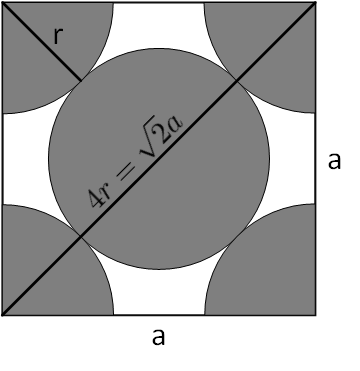
\includegraphics[width=0.3\linewidth]{Graphics/Chapter1/r_a_relation}
	\caption{Relation between the atomic radius and the parameter a in a FFC}
	\label{fig:r_a_relation}
\end{figure}

 As \autoref{fig:r_a_relation} shows the relationship between the parameter $a$ and the radius of the atomic sphere is given as:
$$r = \frac{\sqrt{2}}{4} a $$

And further the volume of the sphere

$$V_{Atom} = \frac{4}{3} \pi r^3 = \frac{a^3 \pi}{\sqrt{2^5}\cdot 3}$$

So the Atomic Packaging Factor $APF$ can be calculated as ratio between the
volume consumed by the atoms to the whole volume.

$$APF = \frac{4 \cdot V_{Atom} }{V_{UC}} = \frac{\pi}{3 \cdot \sqrt{2}} \approx 74\%$$


\textbf{Density}

The atomic mass of calcium us given as:
$$M_{Ca} = 40.078 \frac{g}{mol}$$


$$\rho = \frac{4}{N_A} \cdot \frac{M_{Ca}}{V_{UC}} = 1.55 \frac{g}{cm^3}$$


\textbf{Planes}

In the following the planes $P1: \, (0\overline{3}2)$ and $P2: \,(\overline{1}21)$ are drawn inside the unit cell.
The Miller-Indices of the planes corresbond to the following plane equations:
$$P1: \quad -\frac{1}{3} y + \frac{1}{2} z = 1$$
$$P2: \quad -x +\frac{1}{2} y + z = 1$$

With respect of the fact that all parallel planes have the same Miller-Indices the planes which were drawn are:
$$P1: \quad z = \frac{2}{3}y$$
$$P2: \quad z = x -\frac{1}{2}y$$

\begin{figure}[H]
	\centering
	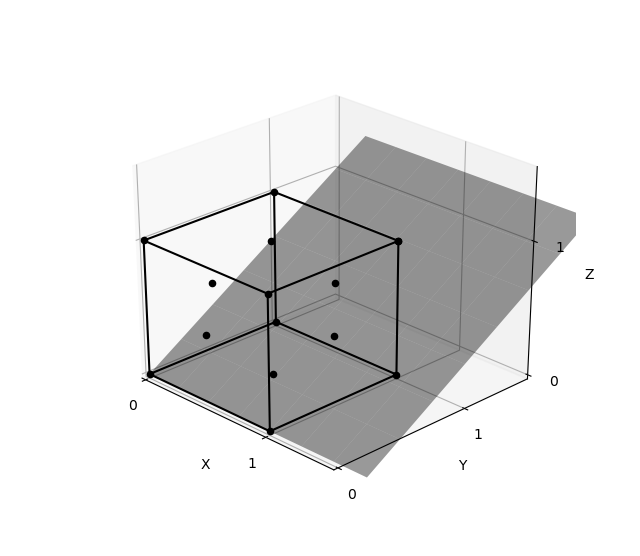
\includegraphics[width=0.6\linewidth]{Graphics/Chapter1/PLANE032}
	\caption{$(0\overline{3}2)$-Plane in a FCC-Lattice}
	\label{}
\end{figure}


\begin{figure}[H]
	\centering
	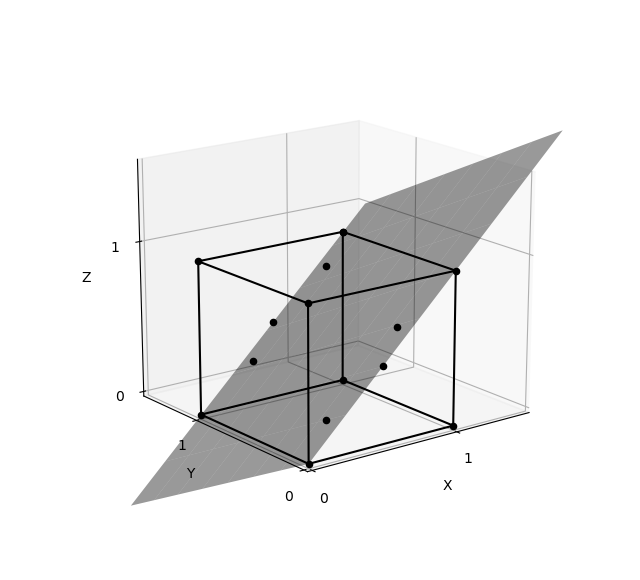
\includegraphics[width=0.6\linewidth]{Graphics/Chapter1/PLANE121}
	\caption{$(\overline{1}21)$-Plane in a FCC-Lattice}
	\label{}
\end{figure}


\textbf{Linear Density [110]}

\begin{figure}[H]
	\centering
	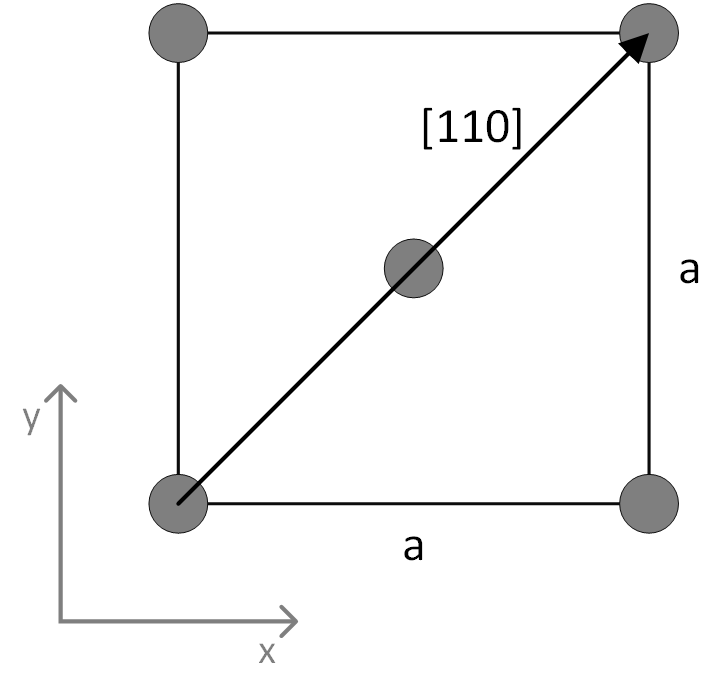
\includegraphics[width=0.5\linewidth]{Graphics/Chapter1/Lin_Den}
	\caption{Linear Density of FCC in [110] Direction}
	\label{Lin_Den}
\end{figure}

\autoref{Lin_Den} shows the [110] direction in a FCC lattice.
As you can see the [110] direction includes 2 atoms inside a 
length of $\sqrt{2}a$.

Therefore  (with $a = 5.56 \, \mathring{A}$)

$$\lambda = \frac{2 \, Atoms}{\sqrt{2}a} = \frac{\sqrt{2}}{5.56} \frac{Atoms}{\mathring{A}}$$

\textbf{Potential Energy}

The potential energy between to adjacent ions can be represented by

\begin{equation}
	E(r) = - \frac{A}{r} + \frac{B}{r^n}
	\label{eq:Pot_Energy}
\end{equation}


To calculate the bonding energy $E_0 = E(r_0)$, which is a minimum of the function $E(r)$,
the derivative has to equals zero.
The negative derivative of the bonding energy equals the interatomic force.

$$F(r) = - \frac{\partial E(r)}{\partial r} = 0$$

$$-\frac{A}{r^2} + \frac{nB}{r^{n+1}} = 0$$
$$\Rightarrow r_0 = \left( \frac{A}{nB} \right)^{\frac{1}{n-1}}$$

By inserting the result for $r_0$ into \autoref{eq:Pot_Energy}, the bonding energy $E_0$ in terms of $A$, $B$ and $n$ results as:

$$E_0 = E(r_0) = - \frac{A}{\left( \frac{A}{nB} \right)^{\frac{1}{n-1}}} + 
				\frac{B}{\left( \frac{A}{nB} \right)^{\frac{n}{n-1}}}$$


		\newpage

		%------2-CHAPTER------%
		\subsection{Chapter 2}

\subsubsection*{Geometric Structure Factor}

The structure factor gives the amplitude of a scattered wave arising
from the atoms with a single primitive cell. 
\begin{equation}
\mathrm{\Phi_k} = \sum_{j} f_j(\mathrm{K)}e^{i\mathrm{K \cdot d}}
\end{equation}
For crystals composed of only one type of atom, it’s common to split
the structure factor into two parts:
\begin{equation}
\mathrm{\Phi_k} = f_j\mathrm(K)S_{\mathrm{K}}
\end{equation}
,where $f_j$ is atomic form factor and $S_\mathrm{K}$ is geometric structure factor. Now let's focus on the second one.
\begin{equation}
S_\mathrm{K} = \sum_{j = 1}^{n} e^{i \mathrm{Kd}}
\end{equation}

For a perfect crystal the lattice gives the reciprocal lattice, which determines the positions (angles) of diffracted beams, and the basis gives the structure factor $F_{hkl}$ which determines the amplitude and phase of the diffracted beams:
\begin{equation}
F_{hkl} = \sum_{j = 1}^{N} f_j \mathrm{e}^{[-2\pi i(hx_j + ky_j + lz_j)]}
\end{equation}

The FCC lattice is a Bravais lattice, and its Fourier transform is a body-centered cubic lattice. However to obtain $F_{hkl}$ without this shortcut, consider an FCC crystal with one atom at each lattice point as a primitive or simple cubic with a basis of 4 atoms, at the origin $ x_j, y_j, z_j = (0, 0, 0)$ and at the three adjacent face centers $ x_j, y_j, z_j = \Big(\frac{1}{2}, \frac{1}{2} , 0\Big), \Big(0, \frac{1}{2} , \frac{1}{2}\Big)\ \mathrm{and}\  \Big(\frac{1}{2} , 0 , \frac{1}{2}\Big) $

$$
F_{hkl} = \sum_{j = 1}^{4} f_j \mathrm{e}^{[-2\pi i(hx_j + ky_j + lz_j)]} = f[1 + (-1)^{h+k} + (-1)^{k+l} + (-1)^{h+l}]
$$

with the result

$$
F_{hkl} = 
\left\{ \begin{array}{ll}
4f, & h,k,l\ $all even or all odd$ \\
0, & h,k,l\ $mixed parity$\\
\end{array} \right.
$$

\begin{itemize}
\item lattice centering (translational operations derived from the lattice type)
\item screw axes (symmetry axes that imply rotation and an additional translation)
\item glide planes (mirror planes that imply reflection and an additional translation).
\end{itemize}


\subsubsection*{Diffraction Maximums}
Bragg diffraction occurs when radiation, with a wavelength comparable to atomic 
spacings, is scattered in a specular fashion by the atoms of a crystalline system, and 
undergoes constructive interference. For a crystalline solid, the waves are scattered 
from lattice planes separated by the interplanar distance $d$. Bragg's law,  describes 
the condition on for the constructive interference to be at its strongest by formula:
\begin{equation}
\label{Bragg}
2d_{hkl} \sin{\theta} =  \lambda
\end{equation}
We need to use the concept of the reciprocal lattice to evaluate the lattice structure
factor $S$, which is involved in the x-ray scattering process. In equation:
\begin{equation}
S = G_{hkl}
\end{equation}
The scattering vector s is equal to a
reciprocal lattice vector.Also this implies that $s$ is normal to the $(hkl)$ crystal planes. For a cubic system we gave also a formula:
\begin{equation}
\frac{1}{d^2} = \frac{h^2 + k^2 + l^2}{a^2}
\end{equation}
After few transformation we get:
$$
d_{hkl} = \frac{a}{\sqrt{h^2 + l^2 + k^2}}
$$
Planes where we obtain a first 3 difraction maximums are following: 
$$P_1 = (111) \qquad P_2 = (200) \qquad P_3 = ( 220) $$  
We can calculate interplanar distances:

$$d_{hkl1} = \frac{5,58}{\sqrt{1^2 + 1^2 + 1^2}} = 3,23 \AA$$
$$d_{hkl2} = \frac{5,58}{\sqrt{2^2 + 0^2 + 0^2}} = 2,79 \AA$$
$$d_{hkl1} = \frac{5,58}{\sqrt{2^2 + 2^2 + 0^2}} = 1,98 \AA$$


\subsubsection*{Reciprocal Lattice}
In order to identify the reciprocal lattice we start by the calculating
the reciprocal lattice vectors, which form a new set of basis vectors.

As in \autoref{chap1} already explained the three primitive vectors
of the fcc structure are:

$$\vec{u} = \frac{a}{2} \left(\begin{matrix}1\\1\\0\\\end{matrix}\right) \qquad
\vec{v} = \frac{a}{2} \left(\begin{matrix}0\\1\\1\\\end{matrix}\right) \qquad
\vec{w} = \frac{a}{2} \left(\begin{matrix}1\\0\\1\\\end{matrix}\right)$$

The new reciprocal lattice vectors are defined as:

\begin{equation}
    \vec{u^*} = \frac{2 \pi}{V_{PC}} (\vec{v} \times \vec{w}) \qquad
    \vec{v^*} = \frac{2 \pi}{V_{PC}} (\vec{w} \times \vec{u}) \qquad
    \vec{w^*} = \frac{2 \pi}{V_{PC}} (\vec{u} \times \vec{v})
\end{equation}

With $V_{PC}$ the volume of the primitive cell given from \autoref{chap1}
as:
$$V_{PC} = \frac{a^3}{4}$$

The three vectors result in:

$$
    \vec{u^*} = \frac{2\pi}{a} \left(\begin{matrix}1\\1\\-1\\\end{matrix}\right) \qquad
    \vec{v^*} = \frac{2\pi}{a} \left(\begin{matrix}-1\\1\\1\\\end{matrix}\right) \qquad
    \vec{w^*} = \frac{2\pi}{a} \left(\begin{matrix}1\\-1\\1\\\end{matrix}\right)
$$

Which represents the primitive translation vectors of a bcc lattice.
Therefore the bcc lattice is the reciprocal lattice to the fcc lattice
in which calcium crystallizes.
		\newpage

		%------3-CHAPTER------%
		\subsection{Lattice Vibrations} \label{chap3}
We start this part with a approximation and treat the solid as a continuous medium.
In reality a solid is composed discrete atoms, however for long wavelength the 
approximation is valid.

\subsubsection*{Density of States (1D)}

We start with the 1-D wave equation:
$$\frac{\partial^2 u}{\partial x^2} - \frac{\rho}{Y} \frac{\partial u}{\partial t} = 0$$

Which delivers a solution in the way of:\\
(The time depence is not needed for calculating the density of states)
\begin{equation}
    u = Ae^{ikx}
    \label{eq:sol_1d_wave}
\end{equation}

By using the boundary conditions:
$$u(x=0) = u(x=L)$$

We get:
$$e^{ikL} = 1$$

Due to Eulers-Equation we get for $k$
$$k = n \frac{2\pi}{L}$$

If you choose integer values for $n$ and plot them along a $k$-axis, they form
an one-dimensional mesh with a constants spacing $(2\pi/L)$ between the points.

\begin{figure}[H]
	\centering
	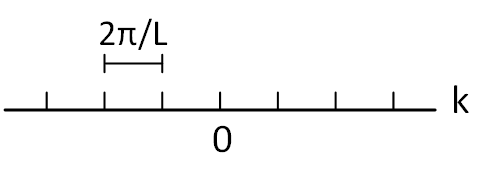
\includegraphics[width=0.4\linewidth]{Graphics/Chapter3/allowed_values_k_1D}
	\caption{Allowed values of $k$}
	\label{}
\end{figure}

As we can see if $L$ becomes large we get quasi-continous points for $k$. So the 
number of modes (points) in an interval $dk$ in $k$-space equals:

$$\dfrac{L}{2\pi} dk$$

Using the dispersion relation we can find the number of modes in a frequency
range $d\omega$, which lies within $(\omega, \omega + d\omega)$.
This number is given as $(g\omega)d\omega$, with
$g(w)$ defined as the density of states.

$$g(\omega) d\omega =\dfrac{L}{2\pi} dk$$

By solving for $g(\omega)$ and multipling with a factor of two.
(Due to the fact that we have to include the modes lying the negative k-region)\\
we get:

\begin{equation}
    g(\omega) = \frac{L}{\pi} \frac{1}{\frac{d\omega}{d k}}
\end{equation}

By assuming that the dispersion in linear $(\omega = v_sk)$ 
the density of states is

\begin{equation}
    g(\omega) = \frac{L}{\pi} \frac{1}{v_s}
\end{equation}

which is independet of $\omega$

\subsubsection*{Density of States (3D)}

Starting with the solution for the wave equation as same as in the 1-D case
(\autoref{eq:sol_1d_wave}) we get:

\begin{equation}
    u = Ae^{i(k_x x + k_y y + k_z z)}
\end{equation}

By applying the same boundary conditions as in the 1-D case we get:

$$u = e^{i(k_x x + k_y y + k_z z)} = 1$$

$$(k_x, \, k_y,\, k_z) = (n \frac{2\pi}{L}, \, m \frac{2\pi}{L}, \, l \frac{2\pi}{L})$$

Each point in this $k$-space has a volume of $(2\pi/L)^3$. The number of
modes that lie within a spherical shell with thickness $dk$ with a radius k 
and a volume $4/3\pi k^3$, is given by:

$$\frac{d}{dk}{(\frac{L}{2\pi})}^3\frac{4}{3}\pi k^3 = {(\frac{L}{2\pi})}^3 4\pi k^2 dk$$

And so with $L^3 = V$:

$$ g(\omega) d \omega =  \frac{V}{2\pi^2} k^2 dk \quad \Rightarrow \quad g(\omega) = \frac{V}{2\pi^2} k^2 \frac{dk}{d \omega} $$

By applying the linear dispersion relation, we get:

\begin{equation}
    g(\omega) = \frac{V}{2\pi^2} \frac{\omega^2}{v_s^3}
    \label{eq:g_ome_3d_1}
\end{equation}

As there are three different modes associated with the same value for $q$
(one longitudinal and 2 transversal modes). \autoref{eq:g_ome_3d_1} has to be
multiplied by a factor of three to get the correct result.

\begin{equation}
    g(\omega) = \frac{3V}{2\pi^2} \frac{\omega^2}{v_s^3}
    \label{eq:g_ome_3d}
\end{equation}

Different to the 1-dimensional case the density of states
in the 3-dimensional case is not a constant, rather increases
as $\omega^2$. This can be explained due to the fact that volume of the 
spherical shell increases with $q^2$ and as $q$ is propotional to 
$\omega$, the dependence on $\omega^2$ can be explained.

\subsubsection*{Debye Frequency}

In the Debye model the vibration frequency of the lattice covers
a wide rang of values.

The total energy of the lattice is calculated by:

\begin{equation}
    E = \int \overline{\epsilon}(\omega) g(\omega) \, d\omega
    \label{eq:debye_energy}
\end{equation}

$g(\omega) \quad ... \quad \textrm{density of states}$\\
$\overline{\epsilon}(\omega) \quad ... \quad \textrm{energy of each mode}$

For various reasons a cutoff frequency is needed for example to not get
infinit energys in \autoref{eq:debye_energy}.

The upper cutoff frequency was defined, by requiring that the total number of 
modes included must be equal to the number of degrees of freedom for the entire
solid.

\begin{equation}
    \int_0^{\omega_D} g(\omega) \, d\omega = 3N_A
    \label{eq:debye_frequency_int}
\end{equation}

With inserting the \autoref{eq:g_ome_3d_1} into equation 
\autoref{eq:debye_frequency_int} the integral can be solved and 
a expression for the Debye frequency $w_D$ is obtained.

$$\int_0^{\omega_D} \frac{3V}{2\pi^2} \frac{\omega^2}{v_s^3} \, d\omega = 
    \frac{3V}{2\pi^2} \frac{1}{v_s^3} \left[\omega\right]_0^{\omega_D} =
    \frac{V}{2\pi^2} \frac{\omega_D^3}{v_s^3}
$$

$$ \frac{V}{2\pi^2} \frac{\omega_D^3}{v_s^3} = 3N_A \qquad \Rightarrow
    w_D = (6\pi^2 n)^{\frac{1}{3}} v_s \textrm{ with } n=\frac{N_a}{V}$$

The debye frequency is proportinal to the 3rd root of the concentration
of the amtos $n$ in the solid. This is simply explained by 3-dimensional 
$q$ space.

\subsubsection*{Monoatomic 1D chain}

We are going to consider elastic vibrations of the atomic network in classic
terms. We assume that:
\begin{enumerate}
\item The average equilibrium position of each atom is placed at the Bravais 
        network node.
\item Atomic deflections from equilibrium positions are small compared to the
        distances between atoms. This assumption leads to harmonic 
        approximation allowing for simplification accounts
\item We will use the Born-Openhaimer adiabatic approximation: the velocities
        of electrons are on the order of $10^8 \mathrm{\frac{cm}{s}}$, while 
        the velocities of nuclei in atoms on the order of at most $10^5 \mathrm
        {\frac{cm}{s}}$. When considering the motion of whole atoms or ions can 
        therefore be assumed that electrons are always in their own
        ground state for a specific atom position.
\end{enumerate}
If the waves propagate in a crystal with a regular structure the entire network planes move in phase, in direction or in parallel or perpendicular to the direction of the wave. After considering every of those statements the frequency of normal vibration modes
$\omega(k)$ of modes with wave vector $k$ (dispersion relationship) can be expressed by:
\begin{equation}
    m\omega^2 = 4K \sin^2\bigg(\frac{ka}{2}\bigg)  
\end{equation}

So $\omega$ is (knwon as the dispersion relationship):

\begin{equation}
    \omega = \sqrt{\frac{4K}{m}}\cdot \vert \sin \left(\frac{ka}{2} \right) \vert
    \label{eq:disp_relation} 
\end{equation}

The group velocity is defined as the partial derivative according to k.

$$v_G = \frac{\partial \omega}{\partial k} = 
     \sqrt{\frac{K}{m}} a \cos\left(\frac{ka}{2} \right)$$

$$v_G(k=0) = \sqrt{\frac{K}{m}} a$$

$$v_G\left(k=-\frac{\pi}{a}\right)= v_G\left(k=\frac{\pi}{a}\right) = 0$$

The group velocities on the edge of the 1 Brillouin zone are zero, which means that we have a standing wave.

\subsubsection*{Disperision Relationship for Calcium}

In \autoref{chap1} we calculated the linear density $\lambda$ for Calcium in the [110]
direction as \autoref{fig:Lin_Den} shows the [110] direction is the 
direction with the lowest distance between the atoms.

Therfore the parameter $a$ in \autoref{eq:disp_relation} is given as the
inverse of the linear density $\lambda$.


Another helpfull relationship is the following:

\begin{equation}
    K = aY = \frac{Y}{\lambda}
\end{equation}
$Y  \quad ... \quad \textrm{Young's modulus}$

Elementary Solid State Physics \cite{elementary_SSP}, p. 91

The Youngs's modulus for calcium can be found in different literature  \cite{web_elem_calcium} and is found to be:

$$Y_{Ca} = 20 GPa$$

So for Calcium the dispersion relationship results in 

\begin{equation}
    \omega(k) = \sqrt{\frac{4 Y_{Ca}}{m_{Ca} \lambda}} \cdot \vert \sin \left(\frac{k}{2\lambda} \right) \vert
\end{equation}
with:
\begin{addmargin}[4em]{1em}
    $Y_{Ca} = 20 GPa$\\
    $m_{Ca} = 40.078 \, u$\\
    $\lambda = \frac{\sqrt{2}}{5.56} \frac{1}{\mathring{A}}$
\end{addmargin}


The resulting graph is shown in \autoref{fig:disp_relat_calcium}.
\begin{figure}[H]
	\centering
	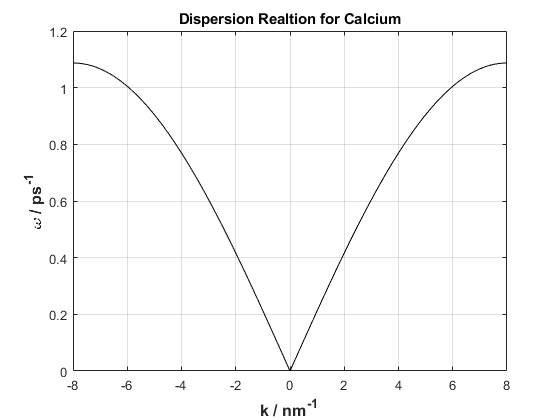
\includegraphics[width=0.7\linewidth]{Graphics/Chapter3/disp_relat_calcium}
	\caption{Disperision Realtion for Calcium}
	\label{fig:disp_relat_calcium}
\end{figure}

\subsubsection*{Experimental methodologies for determining the frequency of the lattice phonons}

The phonon dispersion, which means the relationship between energy and momentum of the 
lattice vibrations can be investigated by inelastic neutron scattering and inelastic 
X-ray scattering. Small pulse phonons which means in the center of the Brillouin zone, 
can be detected by Raman, infrared spectroscopy or Brillouin scattering.

If radiation is used, conservation of momentum requires that

$$\mathbf{k} = \mathbf{k_0} + \mathbf{q}$$

Where $\mathbf{q}$ is the wave vector of the phonon and $\mathbf{k}$
is the scattered wave vector and $\mathbf{k_0}$ the initial wave vector.

Due to the fact of conservation of energy, it is required that
$$\omega = \omega_0 \pm \omega(\mathbf{q})$$
$\omega  \quad ... \quad \textrm{Frequency of the scattered beam}$\\
$\omega_0  \quad ... \quad \textrm{Frequency of the initial beam}$\\
$\omega(\mathbf{q})  \quad ... \quad \textrm{Frequency the phonon}$

This means pratically instead of one diffraction maximum seen at $\omega_0$ 
now two maximum are located symmetrically arroun $w_0$ which can be used 
to determine the frequency of the phonos.

Another way to determining characteristics of phonons is the use of Ultrasonic Waves.
Basic properties like anharmonic interactions and phonon-spin action can be investigated
by ultrasonic phonons of carefully controlled frequency an polarization.

As optical phonons in ionic crystal interacts strongly with light, this properties
could be used to get further insides. Especially in the case of infrared light
strong reflections and absorption appear. As optical phonons exist only in multi-atom
base crystal, it could not be used for a simple $Ca$ crystal, but for example for
$CaF_2$.
		\newpage

	\section{Conclusion}
	This report described Solid-State properties of Calcium. Basic issues describing calcium have been determined like:
\begin{itemize}
\item primitive vectors
\item packaging factor
\item Miller-Indices of the planes
\end{itemize}
and also some more complicated factors:
\begin{itemize}
\item Geometric Structure Factor
\item Reciprocal Lattice
\end{itemize}
To determine which X-ray wavelength should be used to determine a maximum diffraction (spot) there was a need to use Ewald sphere issue. There were also performed some mathematical deductions in order to find density of states. Whole report helps to undarstand basic assumptions of solid state physics.
	\newpage

	\begin{thebibliography}{9}
    \bibitem{elementary_SSP} 
    M.A. Omar, Elementary Solid State Physics:  
    \textit{Principles and Applications}, 
    Addison-Wesley, London, 1993.
    
\end{thebibliography}
	\newpage


	\listoftables
	\listoffigures
\end{document}
